\chapter{Potential Outcomes}
\label{ch-po}
This chapter
is based on Ref.\cite{book-mixtape},
a book by Stephen Cunningham entitled 
``Causal inference: the mixtape".

The theory of potential
outcomes (PO) was for the most part
invented in a seminal
1974 paper by Donald B. Rubin. Rubin
has also
made important extensions
to PO theory since 1974. However, he refuses to
use Pearl's causal DAGs to discuss PO theory. 
Pearl has shown that PO theory
can be substantially clarified
and extended by using
the language of causal DAGs.
The d-separation theorem 
that we discuss in  Chapter \ref{ch-dsep}
is especially
useful in this regard.


In this chapter, we stress the
connection
of PO theory to bnets,
and, in particular, to 
the do and imagine operators 
defined in Chapter \ref{ch-counterf}. Hence,
before reading this chapter,
the reader is expected to have at least
skimmed  Chapter \ref{ch-counterf},
so that he/she understands
the definition
of do and imagine operators.

\begin{table}[h!]
\centering
\begin{tabular}{|l|l|l|l|l|}
\hline
\rowcolor[HTML]{ECF4FF} 
$\s$ & $\rvd^\s$ & $\rvy^\s$ & $\rvy^\s(0)$ & $\rvy^\s(1)$ \\ \hline
Edith & 0 & 5 & 5 & . \\ \hline
Frank & 0 & 7 & 7 & . \\ \hline
George & 0 & 8 & 8 & . \\ \hline
Hank & 0 & 10 & 10 & . \\ \hline
Andy & \cellcolor[HTML]{FFFFC7}1 & 10 & . & 10 \\ \hline
Ben & \cellcolor[HTML]{FFFFC7}1 & 5 & . & 5 \\ \hline
Chad & \cellcolor[HTML]{FFFFC7}1 & 16 & . & 16 \\ \hline
Daniel & \cellcolor[HTML]{FFFFC7}1 & 3 & . & 3 \\ \hline
\end{tabular}
\caption{PO dataset describing whether
individual $\s$
took a treatment dose ($d^\s=1$)
or didn't ($d^\s=0$).
The 
treatment outcome
is measured by the real number $y^\s$.}
\label{tab-pot-out-missing}
\end{table} 

Suppose a {\bf population
of individuals} $\s=0,1,2, \ldots, nsam-1$
is given ($d^\s=1$) or
not given ($d^\s=0$)
a {\bf treatment discrete drug dose} $d^\s$,
and that
the 
 {\bf treatment outcome (i.e., response)}
is measured by
a real number $y^\s$.
Table \ref{tab-pot-out-missing}
gives a possible {\bf PO dataset}
for this scenario.
As you
can see from
that table,
each individual 
either takes a drug
dose or
doesn't,
but not both.
PO theory
can be viewed as a
 {\bf  missing
data (MD) problem}. MD problems are 
discussed in
 Chapter \ref{ch-missing-d}.
However, the PO MD problem 
is much more specialized
than the generic MD problems
discussed in Chapter \ref{ch-missing-d}.
In the PO MD
problem, we can
fill
in the blank cells
by matching
each individual
that took
the drug with
another {\it similar} 
individual that didn't.
We will have much
more to say about
this matching
strategy later in this chapter.

One can define
similar
individuals as 
individuals that have the same
value
for $nx$ features $x^\s=(x^\s_i)_{i=0, 1, \ldots, nx-1}$.
One
can add to Table \ref{tab-pot-out-missing}
 $nx$ extra columns
giving the value of
the feature vector $x^\s$
for each individual.
Members
of a population with
the same $x^\s$ 
are referred to as 
a
{\bf subpopulation or stratum (ie., layer)}.

In a {\bf randomized clinical trial (RCT)},
the effect 
of the variable $x^\s$ on 
the value
of $d^\s$
is eliminated by
randomizing
the population
and therefore
making the effect of $x^\s$
average out  to zero.
However,
there are many situations
in which carrying out an RCT is not
possible. PO theory is
a way of predicting the
result
of an RCT in situations where
doing a real RCT is not physically possible.

In this chapter, $x^\s$
will be called the confounders.
Implicit throughout this chapter
is the assumption that there are {\bf 
no unmeasured confounders}.
Because if 
there are some unmeasured confounders,
those can
send secret messages 
that influence the value 
that $d^\s$ takes.
This would ruin
the
predictions
of someone trying
to predict the results of an RCT
without
being privy to those secret 
messages.
When there are {\bf some
unmeasured confounders},
it might still be
possible
to
predict the effect of an RCT.
This might be possible
using instrumental variables. See Chapter
\ref{ch-instrumental}
for a discussion
of {\bf instrumental
variables}.


\section{$G$ and $G_{den}$,
bnets,
the starting point bnets}


\begin{figure}[h!]
$$
\begin{array}{ccc}
\xymatrix{
&\rvx\sqsig\ar[dl]\ar[dr]
\\
\rvd\sqsig\ar[rr]&&\rvy\sqsig
}
&&
\xymatrix{
u_\rvd\ar[dd]&u_\rvx\ar[d]&u_\rvy\ar[dd]
\\
&\rvx\ar[dl]\ar[dr]
\\
\rvd\ar[rr]&&\rvy
}
\\
\\
G&&G_{den}
\end{array}
$$
\caption{Bnets
$G$ and $G_{den}$
are 
our starting
point in discussing PO theory. 
 $G$ is for 
a single individual $\s$ of the 
population.
Bnet $G_{den}$ is the 
DEN counterpart 
to $G$.
DEN (Deterministic with
External Noise) bnets are discussed in Chapter
\ref{ch-linear-sys}.} 
\label{fig-po-G-start}
\end{figure}

In this chapter, we will
abbreviate
$\rvX\sqsig=\rvX^\s$
for
$X\in \{d, x, y\}$ 
and for $\s=\{0,1,2, \ldots, nsam-1\}$.


For each individual (aka unit, sample) 
$\s=0, 1, 2, \ldots nsam-1$, let:

$\rvd^\s\in\bool$: treatment discrete drug dose,  1 if treated and 0 if untreated

$\rvy^\s\in \RR$:
 treatment potential outcome

$\rvx^\s$: column vector of treatment 
confounders 
(aka covariates, because they
are often used as covariates (i.e., 
independent
variables) in linear regression.)

Consider bnets $G$ and $G_{den}$
in 
 Fig.\ref{fig-po-G-start}.
$G$ reflects the language
used in Ref.\cite{book-mixtape}
to discuss PO theory. And
$G_{den}$ reflects
the language that Judea Pearl 
prefers to use to discuss PO theory.
Both languages are equivalent. To go from
one language to the other, one need only
perform the following
swaps, where $\rvu$
is the external noise of the DEN bnet.

$\rvX^\s\leftrightarrow \rvX(\rvu)$
for $X\in \{d, x, y\}$.

$P(\s)=\frac{1}{nsam}\leftrightarrow P(u)$

$\sum_\s P(\s) (\cdot)
\leftrightarrow \sum_uP(u) (\cdot)$




The TPMs, printed in blue,
for the bnet
$G$
in Fig.\ref{fig-po-G-start},
are as follows:


\beq\color{blue}
P(x^\s)=
P_{\rvx}(x^\s)
\eeq

\beq\color{blue}
P(d^\s|x^\s)=
P_{\rvd|\rvx}(d^\s|x^\s)
\eeq


\beq\color{blue}
P(y^\s|x^\s, d^\s)=
P_{\rvy|\rvx, \rvd}(y^\s|x^\s, d^\s)
\eeq




Now let:

$\rvd\in\bool$: treatment discrete drug dose,  1 if treated and 0 if untreated

$\rvy\in \RR$:
 treatment potential outcome

$\rvx$: column vector of 
treatment
confounders (aka covariates)


$\rvu=(\rvu_\rvd, \rvu_\rvx, \rvu_\rvy)$:
external noise

The TPMs, printed in blue,
for the bnet
$G_{den}$
in Fig.\ref{fig-po-G-start},
are as follows:


\beq \color{blue}
P(x|u_\rvx)= \indi(\;\;x=u_\rvx\;\;)
\eeq

\beq\color{blue}
P(d|x, u_\rvd)=
\indi( \;\; d= f_\rvd(x, u_\rvd)
\;\;)
\eeq

\beq\color{blue}
P(y|d,x, u_\rvy)=
\indi( \;\; y= f_\rvy(d,x, u_\rvy)
\;\;)
\label{eq-y-is-fy}
\eeq

If we linearize
 $f_\rvy$ in Eq.(\ref{eq-y-is-fy}),
we get

\beqa
\rvy =
\delta \rvd + \beta \rvx + \rvu_\rvy
\;,
\label{eq-y-is-lin}
\eeqa
where $\delta, \beta\in \RR$.
Assuming
that $\rvx, \rvy\in \RR$
and $\rvd\in \bool$,
Eq.(\ref{eq-y-is-lin}) can be plotted.
The resulting plot
is given in Fig.\ref{fig-po-two-parallel-lines}.
This plot
is a very special
case of the PO problem,
but it gives a crude idea
of the ``effects" $\delta
= y(1)-y(0)$ that PO theory 
gives estimates for.
Any 
individual participating in the experiment
experiences either $y(1)$
or $y(0)$,
but not both.



\begin{figure}[h!]
\centering
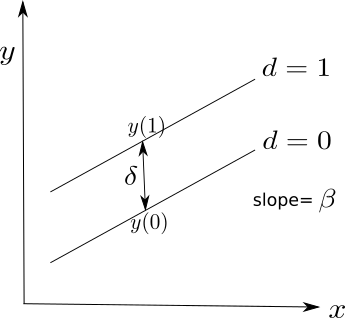
\includegraphics[width=2in]
{pot-out/two-parallel-lines.png}
\caption{Plot  of
Eq.(\ref{eq-y-is-lin})} 
\label{fig-po-two-parallel-lines}
\end{figure}




\section{$G_{do+}$  bnet}
\begin{figure}[h!]
$$
\begin{array}{ccccc}
\xymatrix{
&\rvx^\s\ar[dr]\ar[dl]
\\
\rvd^\s\ar[rr]&&\rvy^\s
}
&&
\xymatrix{
&\rvx^\s\ar[dr]
\\
\rho\rvd^\s=\td^\s\ar[rr]&&\rvy^\s
}
&&
\xymatrix{
&\rvx^\s\ar[dr]
\\
\rho\rvd^\s\ar[rr]&&\rvy^\s
}
\\
\\
G&&G_{do}= \rho_{\rvd^\s}
(\td^\s)G&& G_{do+}
\end{array}
$$
\caption{Bnet $G_{do}= \rho_{\rvd^\s}
(\td^\s)G$
is obtained by applying 
the do operator to node $\rvd^\s$
of bnet $G$. Bnet $ G_{do+}$
is obtained
by adding a prior
probability distribution $P(\td^\s)$
to node $\rho\rvd^\s$ of
bnet $G_{do}$.}
\label{fig-po-G-do}
\end{figure}

Fig.\ref{fig-po-G-do}
shows how bnet $G_{do}$
is obtained by applying 
the do operator to bnet $G$,
and
how
bnet $G_{do+}$
is obtained by adding
a prior
probability distribution
 to one of the nodes
of $G_{do}$.
In bnet $G_{do}$,
node  $\rvd^\s$ has been
stripped of all outside 
influences and fixed to a
specific state $\td^\s$.
This is what an RCT does.

The TPMs, printed in blue,
for the bnets $G_{do}$
and $G_{do+}$,
are as follows.
Note that the TPMs
for bnets  $G_{do}$ and $G_{do+}$
are defined in terms
of the TPMs of bnet $G$.

\beq\color{blue}
P(x^\s)=
P_{\rvx}(x^\s)
\eeq

\beq
P_{\rho\rvd}(d)=\sum_x P_{\rvd|\rvx}
(d|x)P_\rvx(x)
\eeq

\beq\color{blue}
P(\td^\s)=
\left\{
\begin{array}{ll}
\delta(\td^\s, (\td^\s)')& \text{for $G_{do}$}
\\
P_{\rho\rvd}(\td^\s)
& \text{for $G_{do+}$}
\end{array}
\right.
\eeq

\beq\color{blue}
P(y^\s|x^\s, \td^\s)=
P_{\rvy|\rvx, \rvd}(y^\s|x^\s, \td^\s)
\eeq


It is convenient
to define
the following
expected values of
$\rvy^\s$
in terms of the TPMs of
bnet $G_{do+}$:

\beq
\caly_{|\td,x}=E_{\s|\td,x}[\rvy^\s]
\rarrow  E_{\rvy|\td,x}[\rvy]
=
\sum_y yP(y|\td,x)
\eeq


\beq
\caly_{|\td}=E_{\s|\td}[\rvy^\s]
\rarrow E_{y|\td}[\rvy]
=
\sum_x \caly_{|\td,x}P(x)
\eeq

\beq
\caly_{|x}=E_{\s|x}[\rvy^\s]
\rarrow E_{y|x}[\rvy]
=
\sum_{\td} \caly_{|\td,x}P(\td)
\eeq


\beq
\caly=E_\s[\rvy^\s]
\rarrow E_y[\rvy]=\sum_{\td,x}
 \caly_{|\td,x}P_{\rvd|\rvx}(\td|x)P(x)
\eeq

\section{$G_{im+}$ bnet}


\begin{figure}[h!]
$$
\begin{array}{ccccc}
\xymatrix{
&\rvx^\s\ar[dl]\ar[dr]
\\
\rvd^\s\ar[rr]&&\rvy^\s
}
&&
\xymatrix{
&\rvx^\s\ar[dl]\ar[dr]
\\
\rvd^\s&\rvtd^\s=\td^\s\ar[r]&\rvy^\s
}
&&
\xymatrix{
&\rvx^\s\ar[dl]\ar[dr]
\\
\rvd^\s&\rvtd^\s\ar[r]&\rvy^\s
}
\\
\\
G&&G_{im}= \kappa_{\rvd^\s\rarrow\rvy^\s}
(\td^\s)G&&G_{im+}
\end{array}
$$
\caption{Bnet 
$G_{im}= \kappa_{\rvd^\s\rarrow\rvy^\s}
(\td^\s)G$
is obtained by applying 
the imagine operator to arrow 
$\rvd^\s\rarrow\rvy^\s$
of bnet $G$. Bnet $ G_{im+}$
is obtained
by adding a prior
probability distribution $P(\td^\s)$
to node $\rvtd^\s$ of
bnet $G_{im}$.
} 
\label{fig-po-G-im}
\end{figure}

Fig.\ref{fig-po-G-im}
shows how bnet $G_{im}$
is obtained by applying 
an imagine operator to bnet $G$,
and how bnet $G_{im+}$
is obtained  by adding
a prior
probability distribution to
one of the nodes of $G_{im}$.
$\rvd\in \bool$ represents the
dose that a patient 
is told to take by a doctor, and
$\rvtd\in \bool$ represents the 
dose he actually takes.
If $\rvd=\rvtd$, the
patient is compliant,
and if $\rvd\neq\rvtd$, he is
non-compliant.


The TPMs, printed in blue,
for the nodes of bnets $G_{im}$ and $G_{im+}$,
are as follows.
Note that the TPMs
for bnets  $G_{im}$ and $G_{im+}$
are defined in terms
of the TPMs of bnet $G$.
Note that
the prior
$P(\td)$ is not arbitrary;
it's calculated from
the TPMs of bnet $G$.


\beq\color{blue}
P(x^\s)=
P_{\rvx}(x^\s)
\eeq

\beq\color{blue}
P(d^\s|x^\s)=
P_{\rvd|\rvx}(d^\s|x^\s)
\eeq

\beq
\pi_\td=P(\td)=\sum_x P_{\rvd|\rvx}
(\td|x)P_\rvx(x)
\eeq

\beq\color{blue}
P(\td^\s)=
\left\{
\begin{array}{ll}
\delta(\td^\s, (\td^\s)')& \text{for $G_{im}$}
\\
\pi_{\td^\s}
& \text{for $G_{im+}$}
\end{array}
\right.
\eeq


\beq\color{blue}
P(y^\s|x^\s, \td^\s)=
P_{\rvy|\rvx, \rvd}(y^\s|x^\s, \td^\s)
\eeq



\section{$G_{im+}$ bnet
with nodes $y^\sigma(0),
y^\sigma(1)$ added to it.}


\begin{figure}[h!]
$$
\begin{array}{ccccc}
\xymatrix{
&\rvx^\s\ar[ddl]\ar[ddr]
\\
\\
\rvd^\s\ar[rr]&&\rvy^\s
}
&&
\xymatrix{
&\rvx^\s\ar[ddl]\ar[d]\ar[dr]
\\
&\rvy^\s(0)\ar[dr]&\rvy^\s(1)\ar[d]
\\
\rvd^\s&\rvtd^\s=\td^\s\ar[r]
\ar[u]\ar[ur]&\rvy^\s
}
&&
\xymatrix{
&\rvx^\s\ar[ddl]\ar[d]\ar[dr]
\\
&\rvy^\s(0)\ar[dr]&\rvy^\s(1)\ar[d]
\\
\rvd^\s&\rvtd^\s\ar[r]\ar[u]\ar[ur]
&\rvy^\s
}
\\
G&&G_{im}= \kappa_{\rvd^\s\rarrow\rvy^\s}
(\td^\s)G&&G_{im+}
\end{array}
$$
\caption{
Fig.\ref{fig-po-G-im}
with two new nodes $\rvy^\s(0)$
and $\rvy^\s(1)$ added to bnets $G_{im}$
and $G_{im+}$.
} 
\label{fig-po-G-im-y0-y1}
\end{figure}

Consider Fig.\ref{fig-po-G-im-y0-y1},
which was obtained by adding two new
nodes $\rvy^\s(0)$
and $\rvy^\s(1)$
to bnets $G_{im}$
and $G_{im+}$ in
Fig.\ref{fig-po-G-im}.
The
TPMs, printed in blue,
 for bnets $G_{im}$ and $G_{im+}$,
are as follows. Note
that we define them in terms
of the TPMs
for bnet $G$.

\beq\color{blue}
P(x^\s)=
P_{\rvx}(x^\s)
\eeq

\beq\color{blue}
P(d^\s|x^\s)=
P_{\rvd|\rvx}(d^\s|x^\s)
\eeq

\beq
\pi_\td=P(\td)=\sum_x P_{\rvd|\rvx}
(\td|x)P_\rvx(x)
\eeq

\beq\color{blue}
P(\td^\s)=
\left\{
\begin{array}{ll}
\delta(\td^\s, (\td^\s)')& \text{for $G_{im}$}
\\
\pi_{\td^\s}
& \text{for $G_{im+}$}
\end{array}
\right.
\eeq


\beq\color{blue}
P(y^\s(0)|\td^\s, x^\s) = 
P_{\rvy(0)|\rvtd, \rvx}(y^\s(0)|\td^\s, x^\s)
\eeq

\beq\color{blue}
P(y^\s(1)|\td^\s, x^\s) = 
P_{\rvy(1)|\rvtd, \rvx}(y^\s(1)|\td^\s, x^\s)
\eeq


\beqa\color{blue}
P(y^\s|y^\s(0), y^\s(1), \td^\s)=
&=&\color{blue}
\indi(y^\s= \td^\s y^\s(1) + (1-\td^\s)y^\s(0))
\\
&=&\color{blue}
\indi(y^\s= y^\s(\td^\s))
\eeqa

For this bnet,
the following is true:

\beqa
P(y^\s|\td^\s, x^\s)
&=&
\sum_{y^\s(0)}
\sum_{y^\s(1)}
\indi(y^\s= y^\s(\td^\s))
P(y^\s(0)|\td^\s, x^\s)
P(y^\s(1)|\td^\s, x^\s)
\\
&=&
\left\{
\begin{array}{ll}
P_{\rvy(0)|\rvtd, \rvx}(
y^\s|\td^\s, x^\s)&\text{ if }
\td^\s=0
\\
P_{\rvy(1)|\rvtd, \rvx}(
y^\s|\td^\s, x^\s)&\text{ if }
\td^\s=1
\end{array}
\right.
\;.
\label{eq-y-is-y-td}
\eeqa
Note that
$P_{\rvy(0)|\td, x}$
and
$P_{\rvy(1)|\td, x}$
are possibly different functions
and that 
$P_{\rvy|\td, x}$
is defined in terms of both
of them. Eq.\ref{eq-y-is-y-td}
implies that for this bnet,

\beqa
\rvy^\s
&=&
\indi(\td^s=1)\rvy^\s(1)
+\indi(\td^s=0)\rvy^\s(0)
\\
&=&
\td^\s\rvy^\s(1)
+(1-\td^s)\rvy^\s(0)
\\
&=&
\rvy^\s(\td^\s)
\eeqa
These are all different
ways of saying the same thing.

It is convenient
to define
the following
expected values of
$\rvy^\s$
in terms of the TPMs of
bnet $G_{im+}$:

\beq
\caly_{d|\td,x}
=
E_{\s|\td,x}[\rvy^\s(d)]
\rarrow
E_{\rvy|\td,x} [\rvy(d)]
=\sum_{y} P(y(\td)|\td,x) y(\td)
\label{eq-need-positivity}
\eeq

\beq
\caly_{d|\td}
=
E_{\s| \td}[\rvy^\s(d)]
\rarrow
E_{\rvy|\td} [\rvy(d)]
=\sum_x \caly_{d|\td,x}P(x)
\eeq

\beq
\caly_{d|x}
=
E_{\s| x}[\rvy^\s(d)]
\rarrow
E_{\rvy|x} [\rvy(d)]
=\sum_\td \caly_{d|\td,x}P(\td)
\eeq

\beq
\caly_{d}
=
E_{\s}[\rvy^\s(d)]
\rarrow
E_{\rvy} [\rvy(d)]
=\sum_{\td,x}\caly_{d|\td,x} P_{\rvd|\rvx}(\td|x)P(x)
\eeq


$\caly_{0|0}, \caly_{1|1}$
are said to be {\bf factual} 
(indicating compliant patients)
whereas 
$\caly_{0|1}, \caly_{1|0}$
are said to be {\bf counterfactual} 
(indicating non-compliant patients).


\section{Conditional Independence Assumption}

The {\bf Conditional Independence Assumption}
 (CIA)
is said to hold 
 if
\beq
(\rvy^\s(0), \rvy^\s(1),
\rvy^\s,\rvtd^\s)\perp_P\rvd^\s | \rvx^\s
\;.
\label{eq-CIA2}
\eeq
This is satisfied by $G_{im}$. To
prove this, check that

\beq
(\rvy^\s(0), \rvy(1),
\rvy^\s,\rvtd^\s)
\perp_{G_{im}} \rvd^\s|\rvx^\s
\;
\eeq
and then invoke
the d-separation theorem 
(see Chapter \ref{ch-dsep}).

Note that
the following are also true

\beq
(\rvy^\s(0), \rvy(1))
\perp_{G_{im}} \rvtd^\s|\rvx^\s
\;
\eeq

\beq
(\rvy^\s(0), \rvy(1))
\perp_{G_{im}} \rvtd^\s
\;
\eeq
by the d-separation theorem,
because $\rvy^\s$
acts as a collider
on all paths 
from $\rvy^\s(d)$ to $\rvtd^\s$
for $d\in\bool$.
However,

\beq
\rvy^\s\perp_{G_{im}} \rvtd^\s|\rvx^\s
\;\;
\text{ is FALSE.}
\eeq


Note that even though CIA means
 $\rvtd^\s\perp_{G_{im}} \rvd^\s|x^\s$,
this does not mean that $\caly_{d|\td, x}=
\caly_{d|x}$.
The reason is that
$\caly_{d|\td, x} = 
E_{|\td^\s=\td, x}[\rvy^\s(d)]$
so $\caly_{d|\td, x}=
\caly_{d|x}$
if $\rvy^\s(d)\perp_{G_{im}}\rvtd^\s|\rvx^\s$,
which is false.
It is possible for
$\caly_{d|\td, x}=
\caly_{d|x}$ to be true.
We discuss that situation 
in Section \ref{sec-td-ignored}.



\section{${\cal Y}_{|\tilde{d},x}$ and $G_{do}$}

Note that
 $\caly_{d|x}$ and $\caly_{|\td,x}$
are not the same thing.

\beq
\caly_{d|x}=
E_{|x}[\rvy(d)]
\;
\eeq
whereas


\beq
\caly_{|\td,x}=
E_{|\td,x}[\rvy]
\;.
\eeq

\begin{claim}
\beq
\caly_{|\td, x}=\caly_{\td|\td,x}
\eeq
\end{claim}
\proof

\beqa
\caly_{\td|\td,x}
&=&
\td\caly_{1|\td, x}
+
(1-\td)\caly_{0|\td, x}
\\
&=&
\td E_{|\td, x}[\rvy(1)]
+
(1-\td)E_{|\td, x}[\rvy(0)]
\\
&=&
E_{|\td, x}[\td \rvy(1)]+(1-\td)\rvy(0)]
\\
&=&
E_{|\td, x}[\rvy]
\\
&=&
\caly_{|\td, x}
\eeqa
\qed




$\caly_{|\td,x}$
is connected to the do operator as follows.

\beq
\caly_{|\td,x}=
\sum_y y P(\rvy=y|\rho \rvd=\td, \rvx=x)
\;,
\label{eq-y-bar-td}
\eeq
where

\beq
P(\rvy=y|\rho \rvd=\td, \rvx=x)=
P(y|\td,x)
\;.
\eeq
In particular, when
$\rvy$ is binary 
(i.e.,  $\rvy\in\bool$), 
Eq.(\ref{eq-y-bar-td}) becomes

\beq
\caly_{|\td,x}=
P(\rvy=1|\rho\rvd=\td, \rvx=x)
\;.
\eeq


\section{Translation Dictionary}

\begin{table}[h!]
\renewcommand{\arraystretch}{1.5}
\centering
\begin{tabular}{|l|l|}
\hline
\rowcolor[HTML]{ECF4FF} 
In standard PO notation&
In our notation 
(for $G_{im}$ or  $G_{im+}$)\\
\hline
$i$, individual (i.e., unit, sample) index& $\s$ \\ 
\hline 
$D_i=d_i$, treatment dose & $\rvd^\s=d^\s$\\
\hline 
$Y_i=y_i$, treatment outcome& $\rvy^\s=y^\s$ \\ 
\hline 
$X_i=x_i$, treatment confounders& $\rvx^\s=x^\s$ \\ 
\hline
$E[Y_i(d)]$ & 
$E_{\s}[\rvy^\s(d)]=\caly_{d}$ \\
\hline
$E[Y_i|D_i=\td]$ & 
$ E_{\s|\td}[\rvy^\s]=\caly_{|\td}$\\
\hline
$E[Y_i(d)|D_i=\td]$ & 
$E_{\s|\td}[\rvy^\s(d)]=\caly_{d|\td}$\\
\hline
$E[Y_i(d)|D_i=\td, X_i=x]$ & 
$E_{\s|\td,x}[\rvy^\s(d)]=\caly_{d|\td,x}$\\
\hline
\end{tabular}
\caption{Dictionary for 
translating
from standard PO notation
of Ref.\cite{book-mixtape} to our notation.
}
\label{tab-pot-out-dict}
\end{table}
\renewcommand{\arraystretch}{1}

Table \ref{tab-pot-out-dict}
gives a dictionary for 
translating
from the standard PO notation 
of Ref.\cite{book-mixtape}
to our notation. $d,\td\in \bool$.
I find
 the standard PO notation 
confusing because it often uses $D_i$
to represent two different nodes, 
$\rvd^\s$ and $\rvtd^\s$ in $G_{im+}$. This confusion
becomes particularly distressing
when we are told in PO notation that

\beq Y_i(d)=d Y_i(1) + (1
-d)Y_i(0)\;,
\eeq
and

\beq
E\left[Y_i(d)|D_i=\td, X_i=x\right]
=\caly_{d|\td,x}
\;.
\eeq
In our notation,
this is saying that

\beq 
\rvy^\s(d)= d \rvy^\s(1) +
 (1-d)\rvy^\s(0)
\;,
\eeq
and

\beq
E_{\s|\rvtd^\s=\td, \rvx^\s=x}
[\rvy^\s(d)]=
\caly_{d|\td,x}
\label{eq-caly-def-ev}
\;.
\eeq



\section{${\cal Y}_{d|\tilde{d}}$
differences (aka treatment effects)}



\begin{figure}[h!]
\centering
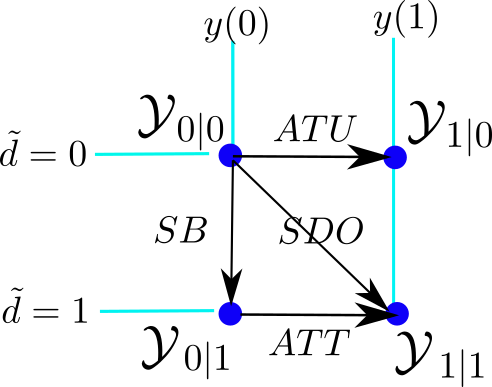
\includegraphics[width=2in]
{pot-out/y-diffs-square.png}
\caption{Different treatment effects.  
An effect is a difference of 
two $\caly_{d|\td}$.} 
\label{fig-y-diffs-square}
\end{figure}

It is convenient to
define the following 
{\bf treatment effects}. 
See Fig.\ref{fig-y-diffs-square}.
Note
that we use  the
word {\bf ``effect"} to
refer to 
a difference of two  $\caly_{d|\td}$.

\begin{itemize}

\item average controlled
causal effect  
 (ACE), used when doing an RCT.

\beq
{\color{red}ACE}=
\caly_{|1}-
\caly_{|0}
=
\caly_{1|1}-
\caly_{0|0}=SDO
\eeq

\item average treatment effect\footnote{
Note that effects in which $\td$ varies
are called
``controlled",
whereas those in which $d$ varies instead,
 are called simply ``treatments".
$y$ is averaged over
in both cases.}
 (ATE).
\beq
{\color{red}ATE}=
\caly_{1}-
\caly_{0}= \delta
\eeq

\item average treatment effect 
of the treated (ATT)
\beq
{\color{red}ATT}=
\caly_{1|1}-\caly_{0|1}
\eeq

\item average
treatment effect of the untreated (ATU)
\beq
{\color{red}ATU}=
\caly_{1|0}-\caly_{0|0}
\eeq


\item selection bias (SB)
\beq
{\color{red}SB}=\caly_{0|1}-\caly_{0|0}
\eeq

\item simple difference in outcomes (SDO)
\beq
{\color{red} SDO}= \caly_{1|1}-\caly_{0|0}
\eeq

\end{itemize}

Note that some
of these effects  are
linearly related



\beq
\underbrace{\caly_1-\caly_0}_
{ATE}=
 \underbrace{(\caly_{1|1}-\caly_{0|1})}_{ATT}\pi_1+
 \underbrace{(\caly_{1|0}-\caly_{0|0})}_{ATU}\pi_0
\eeq

\beq
\underbrace{\caly_{1|1}-\caly_{0|0}}_{SDO}
=
\underbrace{(\caly_{1|1}-\caly_{0|1})}_{ATT}
+
\underbrace{\caly_{0|1}-\caly_{0|0}}_{SB}
\eeq

\beqa
\underbrace{\caly_{1|1}-\caly_{0|0}}_{SDO}
&=&
\underbrace{(\caly_{1|1}-\caly_{0|1})\pi_1 +
(\caly_{1|0}-\caly_{0|0})\pi_0 }_{ATE} 
\\
&&+
\underbrace{\caly_{0|1}-\caly_{0|0}}_{SB}
\\
&&+
\underbrace{(\caly_{1|1}-\caly_{0|1})}_{ATT}\pi_0
\\
&&-
\underbrace{(\caly_{1|0}-\caly_{0|0})}_{ATU}\pi_0
\eeqa


Let $\cale \in\{ACE,ATE,ATT,ATU,SDO, SB\}$.
$\cale$ can be 
defined for a fixed stratum $x$
by replacing $\caly_{d|\td}$
with  $\caly_{d|\td, x}$. 
We will denote such
an extension by $\cale_{|x}$,
or, sometimes, simply by $\cale$.
ATE$_{|x}$ is sometimes called 
the {\bf Conditional
Average Treatment Effect (CATE)}.
We will use the term
ATE to refer to CATE too.\footnote{Careful:
We define
$
ATE_{|x}= ATT_{|x} P_{\rvd|\rvx}(1|x) +
ATU_{|x} P_{\rvd|\rvx}(0|x) 
$. Therefore,
$
ATE_{|x}\neq ATT_{|x} P_{\rvd}(1) +
ATU_{|x} P_{\rvd}(0) 
$.
}



\section{Zero ACE, $\caly_{1|0}=\caly_{1}$}
\label{sec-td-ignored}

\begin{figure}[h!]
\centering
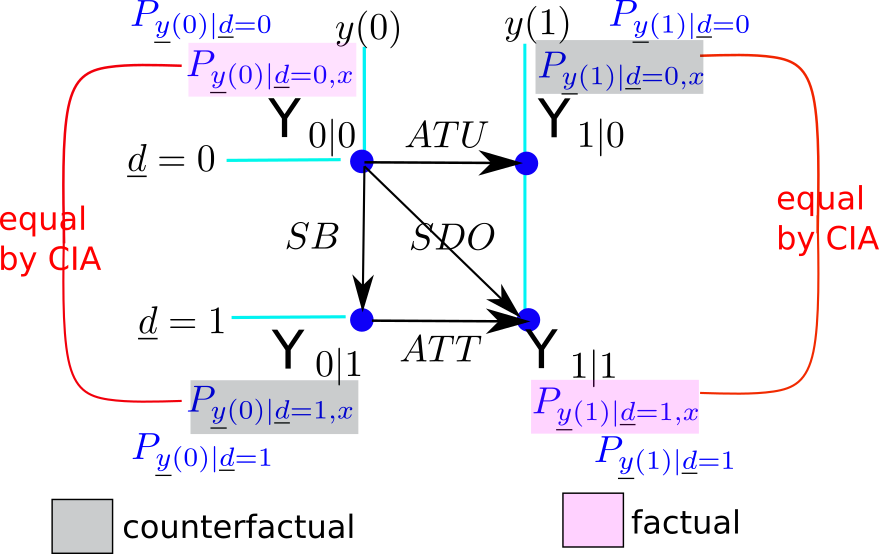
\includegraphics[width=2.5in]
{pot-out/y-diffs-square-probs.png}
\caption{Figure \ref{fig-y-diffs-square} 
with added information
about  probability distributions 
used to obtain each expected value $\caly_{d|\td}$.}
\label{fig-y-diffs-square-probs}
\end{figure}

$ACE=0$
is the hypothesis 
tested by a Randomized Control Trial (RCT).
But some people
test for $ATE=0$
instead.
Is it
possible for $ACE=0$ but $ATE\neq 0$
or vice versa, and
what is going on when this is true?
When is $\caly_{1|0}=\caly_{1}$,
and what is going on when this is  true?
Fig.\ref{fig-y-diffs-square-probs}
gives some 
intuition 
about what is
going on when these 
things happen.

Recall that
each expected value $\caly$ has a probability
distribution $P$.
\beq
\caly_{d|\td, x}=\sum_{y} y P_{\rvy(d)|\rvtd, \rvx}(y|\td,x)
\eeq
for $d, \td\in \bool$.
Fig.\ref{fig-y-diffs-square-probs}
reminds us of which $P$
is used to generate each $\caly$.
From this figure, we see that
a sufficient
condition for $ACE=SDO=0$
is that 
$P_{\rvy(1)|\rvtd=1, \rvx}
=
P_{\rvy(0)|\rvtd=0, \rvx}$.
Also, since $ATE=0$ iff 
$ATT=ATU=0$,
a sufficient condition
for $ATE=0$ is that
$P_{\rvy(1)|\rvtd=0, \rvx}
=
P_{\rvy(0)|\rvtd=0, \rvx}$
and
$P_{\rvy(1)|\rvtd=1, \rvx}
=
P_{\rvy(0)|\rvtd=1, \rvx}$.
Also, 
if we assume that
all $y^\s>0$, $\caly_{1|0}=\caly_{1}$
iff 
$P_{\rvy(1)|\rvtd=0, \rvx}=
P_{\rvy(1)| \rvx}$.
$ACE=0$
depends on two corners
of the square
whereas  $\caly_{1|0}=\caly_{1}$
depends on just one corner.




\section{Matching Strata}

For a situation
described by
the bnet $G_{im+}$,
we can match {\it similar}
individuals to fill the blank cells of
 Table \ref{tab-pot-out-missing}.
By ``similar", we mean that
they have the same or almost the same
value of $\rvx^\s$.


\subsection{Exact strata-match}

For $\td\in \bool$ and all strata $x$,
define the sets of individuals
$A_{\td,x}=\{\s: \td^\s=\td, x^\s=x\}$,
$A_x=A_{0,x}\cup A_{1,x}$ and $A=\cup_x A_x$.
Let $N_{d,x}=size(A_{d,x})$,
$N_x= size(A_x)$ and $N=size(A)$.

In an exact strata-match,
we match each individual with
$\td^\s=1, x^\s=x$
with
exactly
one individual
with $\td^\s=0, x^\s=x$
and vice versa.
Define a map $s:A\rarrow A$
such that,
for each $x$,
$s(A_{0,x})\subset A_{1,x}$ and
$s(A_{1,x})\subset A_{0,x}$.
This assumes $A_{0,x}$ and $A_{1,x}$
are non-empty for all $x$.
The purpose of map $s()$
is
to fill in the missing data in the
PO dataset. See Fig.\ref{tab-po-s-map}
for a pictorial representation of 
this.

\begin{table}[h!]
\centering
\begin{tabular}{|l|l|l|}
\hline
 & \cellcolor[HTML]{ECF4FF}$y^\s(0)$ & \cellcolor[HTML]{ECF4FF}$y^\s(1)$ \\ \hline
\cellcolor[HTML]{ECF4FF}$\td^\s=0$ & $y^\s$ & $y^{s(\s)}$ \\ \hline
\cellcolor[HTML]{ECF4FF}$\td^\s=1$ & $y^{s(\s)}$ & $y^\s$ \\ \hline
\end{tabular}
\caption{Illustration of the
purpose of the map $s()$.
Note that $y^\s=y^\s(\td^\s)$ and $y^{s(\s)}=y^\s(!\td^\s)$,
where $!0=1$ and $!1=0$.}
\label{tab-po-s-map}
\end{table}


Note that

\beq
E_{|x}[\rvtd^\s \rvy^\s]\neq
E_{|x}[\rvtd^\s]\;\;E_{|x}[ \rvy^\s]
\eeq
but
\beq
E_{|x}[\rvd^\s \rvy^\s]=
E_{|x}[\rvd^\s]\;\;E_{|x}[ \rvy^\s]
\eeq
because, by d-separation, at fixed $x$,
 $\rvy^\s$ and $\rvtd^\s$
are not independent 
but $\rvy^\s$ and $\rvd^\s$ are.
Table \ref{tab-po-quadrants}
evaluates various
expected values of the type
 $E_{|x}[\rvtd^\s \rvy^\s]$.


\renewcommand{\arraystretch}{1.5}
\begin{table}[h!]
\centering
\begin{tabular}{|l|l|l|}
\hline
 & \cellcolor[HTML]{ECF4FF}$y^\s(0)$ & \cellcolor[HTML]{ECF4FF}$y^\s(1)$ \\ \hline
\cellcolor[HTML]{ECF4FF}$\td^\s=0$ & \begin{tabular}[c]{@{}l@{}}$E_{|x}[(1-\rvtd^\s) \rvy^\s]=E[1-\rvtd^\s]\caly_{0|0,x}$\\ $E_{|x}\left[\frac{1}{N_{0,x}}\sum_{\s\in A_x} (1-\rvtd^\s)\rvy^{\s}\right]=\caly_{0|0,x}$\end{tabular} & \begin{tabular}[c]{@{}l@{}}$E_{|x}[(1-\rvtd^\s )\rvy^{s(\s)}]=E[1-\rvtd^\s]\caly_{1|0,x}$\\ $E_{|x}\left[\frac{1}{N_{0,x}}\sum_{\s\in A_x} (1-\rvtd^\s) \rvy^{s(\s)}\right]=\caly_{1|0,x}$\end{tabular} \\ \hline
\cellcolor[HTML]{ECF4FF}$\td^\s=1$ & \begin{tabular}[c]{@{}l@{}}$E_{|x}[\rvtd^\s \rvy^\s]=E[\rvtd^{s(\s)}]\caly_{0|1,x}$\\ $E_{|x}\left[\frac{1}{N_{1,x}}\sum_{\s\in A_x} \rvtd^\s \rvy^{s(\s)}\right]=\caly_{0|1,x}$\end{tabular} & \begin{tabular}[c]{@{}l@{}}$E_{|x}[\rvtd^\s \rvy^\s]=E[\rvtd^\s]\caly_{1|1,x}$\\ $E_{|x}\left[\frac{1}{N_{1,x}}\sum_{\s\in A_x} \rvtd^\s \rvy^\s\right]=\caly_{1|1,x}$\end{tabular} \\ \hline
\end{tabular}
\caption{Expected Values
of the type
 $E_{|x}[\rvtd^\s \rvy^\s]$.}
\label{tab-po-quadrants}
\end{table}
\renewcommand{\arraystretch}{1}


Recall that

\begin{subequations}
\label{eq-to-estimate}

\beq
ACE = SDO
\eeq

\beq
ATE = ATT \;\;P_{\rvd|\rvx}(1|x) + ATU \;\;P_{\rvd|\rvx}(0|x)
\eeq

\beq
ATT=
\caly_{1|1,x}-\caly_{0|1,x}
\eeq

\beq
ATU=
\caly_{1|0,x}-\caly_{0|0,x}
\eeq

\beq
SB=\caly_{0|1,x}-\caly_{0|0,x}
\eeq


\beq
SDO=\caly_{1|1,x}-\caly_{0|0,x}
\eeq

\end{subequations}

Eqs.(\ref{eq-to-estimate})
can be estimated from the data
via the following estimators.


\beq
\widehat{ACE} = \widehat{SDO}
\label{eq-est-ace}
\eeq

\beqa
\widehat{ATE}
&=&
\frac{1}{N_x}[
\widehat{ATT}N_{1,x} + 
\widehat{ATU}N_{0,x}]
\\
&=&
\frac{1}{N_x}
\left[\sum_{\s\in A_x} \td^\s [y^\s - y^{s(\s)}]+
\sum_{\s\in A_x}(1-\td^\s) [ y^{s(\s)}-y^\s]
\right]
\\
&=&
\frac{1}{N_x}\sum_{\s\in A_x} (2\td^\s-1)[y^\s -y^{s(\s)}]
\label{eq-est-ate}
\eeqa

\beqa
\widehat{ATT}
&=&
\overbrace{\frac{1}{N_{1,x}}\sum_{\s\in A_x} \td^\s y^\s}^{\caly_{1|1,x}}
 - 
\overbrace{\frac{1}{N_{1,x}}\sum_{\s\in A_x} \td^\s y^{s(\s)}}^{\caly_{0|1,x}}
\\
&=&
\frac{1}{N_{1,x}}\sum_{\s\in A_x} \td^\s [y^\s - y^{s(\s)}]
\label{eq-est-att}
\eeqa


\beqa
\widehat{ATU}
&=&
\overbrace{\frac{1}{N_{0,x}}\sum_{\s\in A_x} (1-\td^\s) y^{s(\s)} }^{\caly_{1|0,x}}
 - 
\overbrace{\frac{1}{N_{0,x}}\sum_{\s\in A_x} (1-\td^\s)y^\s}^{\caly_{0|0,x}}
\\
&=&
\frac{1}{N_{0,x}}\sum_{\s\in A_x} (1-\td^\s) [ y^{s(\s)}-y^\s]
\label{eq-est-atu}
\eeqa

\beq
\widehat{SB} =
\overbrace{\frac{1}{N_{1,x}}\sum_{\s\in A_x} \td^\s y^{s(\s)}}^{\caly_{0|1,x}}
-
\overbrace{\frac{1}{N_{0,x}}\sum_{\s\in A_x} (1-\td^\s)y^\s}^{\caly_{0|0,x}}
\label{eq-est-sb}
\eeq

\beq
\widehat{SDO}=
\overbrace{\frac{1}{N_{1,x}}\sum_{\s\in A_x} \td^\s y^\s}^
{\caly_{1|1,x}}
-
\overbrace{\frac{1}{N_{0,x}}\sum_{\s\in A_x} (1-\td^\s) y^\s}^
{\caly_{0|0,x}}
\label{eq-est-sdo}
\eeq



Let 

\beq
g_d(x)=P_{\rvd|\rvx}(d|x)
\eeq
 for $d\in\bool$.
Note that $g_0(x)+g_1(x)=1$.
$g_1(x)$ is called the {\bf propensity score}.
One can do {\bf propensity weighting}
within the above estimators to
improve their behavior.
This is done by making the
following replacements.

\beq
N_{1,x}
\rarrow
N_x g_1(x^\s)
\;,\;\;
N_{0,x}
\rarrow
N_x g_0(x^\s)
\;.
\eeq
These replacements are
equal under $ \sum_{\s\in A_x}$
to the terms they replace.


\subsubsection{Example, calculation
of
estimators for a treatment}


For $\s\in \{1,2, \ldots, 10\}$, define

\beq
s(\s)=
\left\{
\begin{array}{ll}
\s+5&\text{if }\s\leq 5
\\
\s-5&\text{if }\s >5
\end{array}
\right.
\eeq


\renewcommand{\arraystretch}{1.5} 

\begin{table}[h!]
\centering
\begin{tabular}{|l|l|l|l|l|l|l|}
\hline
\cellcolor[HTML]{ECF4FF} $\s$& \cellcolor[HTML]{ECF4FF}$\td^\s$ & \cellcolor[HTML]{ECF4FF}$y^\s$ & \cellcolor[HTML]{ECF4FF}$\td^\s y^\s$ & \cellcolor[HTML]{ECF4FF}$(1-\td^\s)y^\s$ & \cellcolor[HTML]{ECF4FF}$\td^\s y^{s(\s)}$ & \cellcolor[HTML]{ECF4FF}$(1-\td^\s)y^{s(\s)}$ \\ \hline
\cellcolor[HTML]{ECF4FF}1 & \cellcolor[HTML]{FFFFC7}0 & 0 & \cellcolor[HTML]{FFFFC7}0 & 0 & \cellcolor[HTML]{FFFFC7}0 & 0 \\ \hline
\cellcolor[HTML]{ECF4FF}2 & \cellcolor[HTML]{FFFFC7}0 & 0 & \cellcolor[HTML]{FFFFC7}0 & 0 & \cellcolor[HTML]{FFFFC7}0 & 1 \\ \hline
\cellcolor[HTML]{ECF4FF}3 & \cellcolor[HTML]{FFFFC7}0 & 1 & \cellcolor[HTML]{FFFFC7}0 & 1 & \cellcolor[HTML]{FFFFC7}0 & 1 \\ \hline
\cellcolor[HTML]{ECF4FF}4 & \cellcolor[HTML]{FFFFC7}0 & 1 & \cellcolor[HTML]{FFFFC7}0 & 1 & \cellcolor[HTML]{FFFFC7}0 & 1 \\ \hline
\cellcolor[HTML]{ECF4FF}5 & \cellcolor[HTML]{FFFFC7}0 & 1 & \cellcolor[HTML]{FFFFC7}0 & 1 & \cellcolor[HTML]{FFFFC7}0 & 1 \\ \hline
\cellcolor[HTML]{ECF4FF}6 & 1 & 0 & 0 & \cellcolor[HTML]{FFFFC7}0 & 0 & \cellcolor[HTML]{FFFFC7}0 \\ \hline
\cellcolor[HTML]{ECF4FF}7 & 1 & 1 & 1 & \cellcolor[HTML]{FFFFC7}0 & 0 & \cellcolor[HTML]{FFFFC7}0 \\ \hline
\cellcolor[HTML]{ECF4FF}8 & 1 & 1 & 1 & \cellcolor[HTML]{FFFFC7}0 & 1 & \cellcolor[HTML]{FFFFC7}0 \\ \hline
\cellcolor[HTML]{ECF4FF}9 & 1 & 1 & 1 & \cellcolor[HTML]{FFFFC7}0 & 1 & \cellcolor[HTML]{FFFFC7}0 \\ \hline
\cellcolor[HTML]{ECF4FF}10 & 1 & 1 & 1 & \cellcolor[HTML]{FFFFC7}0 & 1 & \cellcolor[HTML]{FFFFC7}0 \\ \hline
\end{tabular}
\caption{Estimators of treatment effects
are calculated for this example. }
\label{tab-po-example}
\end{table}
\renewcommand{\arraystretch}{1}


\begin{table}[h!]
\centering
\begin{tabular}{|
>{\columncolor[HTML]{ECF4FF}}l |l|l|}
\hline
\cellcolor[HTML]{CBCEFB}$N(\td, y)$ & \cellcolor[HTML]{ECF4FF}$y=0$ & \cellcolor[HTML]{ECF4FF}$y=1$ \\ \hline
$\td=0$ & 2 & 3 \\ \hline
$\td=1$ & 1 & 4 \\ \hline
\end{tabular}
\caption{$N(\ul{\td^\s}=d, \rvy^\s=y)$ for
the data in Table \ref{tab-po-example}.}
\label{tab-n-po-example}
\end{table}

Let $N(\cals)$
be the number of individuals $\s$
that satisfy condition $\cals$.
For example, 
$N(\ul{\td^\s}=\td)$
is the number of individuals
such that $\ul{\td^\s}=\td$.

\beq
N_1
=
N(\td^\s=1)
=
5
\eeq

\beq
N_0
=
N(\td^\s=0)
=
5
\eeq

\beq
N
= N_0+N_1
=
10
\eeq



\beq
\caly_{1|1}
=
\frac{1}{N_1}
\sum_\s \td^\s y^\s
=
\frac{4}{5}
\eeq

\beq
\caly_{0|0}
=
\frac{1}{N_0}
\sum_\s (1-\td^\s) y^\s
=
\frac{3}{5}
\eeq

\beq
\caly_{0|1}
=
\frac{1}{N_1}
\sum_\s \td^\s y^{s(\s)}
=
\frac{3}{5}
\eeq

\beq
\caly_{1|0}
=
\frac{1}{N_0}
\sum_\s (1-\td^\s) y^{s(\s)}
=
\frac{4}{5}
\eeq

\beq
ATT=
\caly_{1|1}-\caly_{0|1}
=\frac{1}{5}
\eeq

\beq
ATT=ATU=ATE=SDO=\frac{1}{5}
\;,\;\; SB=0
\eeq

This example is unusual
in that it has a single
stratum $x$, and for
that stratum, 
the treated and 
untreated populations
are {\bf balanced} (of equal size).
Also, the map $s()$
is 1-1 onto.
If, for instance,
$s(\s)=6$ for all $\s\in A_0$
and $s(\s)=5$ for $\s\in A_1$,
then $ATT, ATU, ATE, SDO$
would not all be same, and 
$SB$ would not be zero.  

\subsection{Approximate strata-match}

It is very often
the case that
one can't
find for a given
individual $\s$
another individual that has
opposite $d^\s$ but
exactly the same value of $x^\s$.
In such cases, one can discard all
matchless individuals.
But that would entail a loss 
of precious information.
Instead of discarding orphans, 
a better way is to
relax our demands and
match individual $\s$
with another individual $s(\s)$
such that $x^\s$
and $x^{s(\s)}$ are very
close in some metric.
Alternatively, the matching
individual might 
not be real; it might
be a composite
of individuals.

More precisely, 
for some arbitrary
parameter $\eps>0$,
and an individual $\s$
with $d^\s=1$,
define
the {\bf strata-matching set} 
$\calm_{\eps}(\s)$ by\footnote{
One can use an $\eps$
that depends on $\s$.
Let $\eps(\s, 5)$
be the radius necessary
so that $\calm_{\eps(\s, 5)}(\s)$
contains exactly 5 elements $s$.
Thus, $\calm_{\eps(\s, 5)}(\s)$
contains the $s$ of the
 5 points $x^s$ that are the
nearest neighbors of $x^\s$
in the $dist()$ metric.}

\beq
\calm_{\eps}(\s)=
\{s: d^\s=1, d^s=0, 
dist(x^\s, x^s)\leq \eps \}
\;,
\eeq
where

\beq
dist(x^\s, x^s)=
[x^\s]^T [\Sigma]^{-1} x^s
\;,
\eeq
where $\Sigma = \av{\rvx^\s, [\rvx^s]^T}$.
 This
metric $dist(x^\s, x^s)$ is
called the {\bf Mahalanobis distance}.
We will call
the case $\eps=0$ an {\bf  exact strata-match},
and
the case
$\eps\neq 0$ 
 an {\bf approximate strata-match.}.
To do an approximate strata-match,
replace $y^{s(\s)}$ 
by
$\av{y}^\s$ 
in 
the estimators 
given above 
for an exact strata-match.
$\av{y}^\s$ 
is defined by

\beq
\av{y}^\s=
\frac{1}{|\calm_{\eps}(\s)|}
\sum_{s\in \calm_{\eps}(\s)}
y^s
\;.
\eeq

Ref.\cite{book-mixtape}
calculates the mean and variance
of estimator $\widehat{ATT}$. 
The mean is biased,
but one can define a new
bias-corrected estimator.


\subsection{Positivity}


{\bf Positivity} is defined as the
requirement that for all layers $x$,
\beq
0<P(d^\s=1|x^\s=x)<1
\eeq
or, equivalently, 
\beq
P(d^\s=1|x^\s=x)>0\text{\;\;\;and
\;\;\;}P(d^\s=0|x^\s=x)>0
\;.
\eeq
In other words, 
for each layer $x$,
there is
a non-zero
probability of being both treated 
and untreated.

Recall that

\beq
\caly_{d|\td,x}
=\sum_{y} y P_{\rvy(d)|\rvtd, \rvx}(y|\td,x)
\;.
\eeq
Also recall
that the estimator
Eq.(\ref{eq-est-att})
for $ATT_{|x}$ divides by $N_{1,x}=P(d=1|x)N_x$
and 
the estimator
Eq.(\ref{eq-est-atu})
for $ATU_{|x}$ divides by $N_{0,x}= P(d=0|x)N_x$.
The estimator Eq.\ref{eq-est-ate}
for $ATE_{|x}$ divides by neither $N_{0,x}$
nor $N_{1,x}$ so it is safe.

If positivity is violated,
then 
for some 
layer $x$, 
 $\caly_{d|\td=0,x}$ or $\caly_{d|\td=1,x}$ 
is undefined. 
Furthermore,  the estimator
$ATT_{|x}$ or $ATU_{|x}$ is undefined.
If $ATT_{|x}$ (or any
other treatment effect)  can be estimated,
one says it is {\bf identifiable} (i.e.,
calculable). If Positivity is violated, then
either $ATT_{|x}$ or $ATU_{|x}$ is not identifiable.

 

When 
$P(d^\s|x^\s=x)$ 
becomes 0 or 1 for some $x$,
the arrow
$\rvx\rarrow\rvd$
becomes deterministic
for some $x$.
This situation
is
the very 
antithesis
of RCTs,
wherein 
the influence
exerted by $\rvx^\s$ on 
$\rvd^\s$ is uniformly
random and therefore ignorable.
Hence, it is perhaps 
not too surprising
that a violation
of positivity makes
$ATT$ or $ATU$
non-identifiable.



\section{Propensity Score}

It is often the case
that the discrete vector $\rvx^\s$
has
too many possible values to make
matching possible.
In such cases, it
is convenient to 
map the space
of vectors
$\rvx^\s$
to the real line.
One very  
convenient choice
for that map
is the 
{\bf propensity score},
which is defined as

\beq
g(x^\s)=P(d^\s=1|x^\s)
\;.
\eeq
The
propensity
score
is usually
approximated
by a sigmoid
function
using logistic regression\footnote{
The sigmoid function is defined
in Chapter \nameref{ch-not-cons}
to be $\sig (x) = 1/(1-e^{-x})$.}

\beq
g(x^\s)= \sig(\alp + \beta x^\s)
\eeq


\begin{figure}[h!]
$$
\xymatrix{
\rvg^\s\ar[d]
&\rvx^\s\ar[dr]\ar[l]
\\
\rvd^\s&\rvtd^\s\ar[r]&\rvy^\s
\\
&G_{ps}
}
$$
\caption{Bnet $G_{ps}$
used when doing propensity scoring.} 
\label{fig-po-G-ps}
\end{figure}
To use the 
propensity score,
one replaces the bnet $G_{im+}$
by the bnet $G_{ps}$
shown in Fig.\ref{fig-po-G-ps}.
The TPMs, printed in blue,
for the 2 nodes of $G_{ps}$
that differ from the nodes
of $G_{im+}$,
are as follows:


\beq\color{blue}
P(g^\s|x^\s)= 
\delta(g^\s, g(x^\s))
\eeq

\beq\color{blue}
P(d^\s|g^\s)= 
g^\s d^\s + (1-g^\s)(1-d^\s)
\eeq

Note that
these TPMs are self-consistent because

\beqa
P(d|x)&=&
\sum_g P(d|g)P(g|x)
\\
&=&
g(x)d + [1-g(x)](1-d)
\\
&=&
P(d=1|x)d + [1-P(d=1|x)](1-d)
\\
&=&
P(d|x)
\eeqa


We would like to do
{\bf propensity score strata-matching} by
matching g-strata instead of x-strata.
 PO calculations
for x-strata matching
use the TPMs
for $P(d|x)$, $P(x)$
and $P(y|d,x)$.
To do g-strata matching
using the same
equations, but 
with $x$ replaced by $g$,
we would need to solve for
$P(d|g)$, $P(g)$
and $P(y|d,g)$
in terms of
$P(d|x)$, $P(x)$
and $P(y|d,x)$.
We solve for those next.

From the TPMs
for $G_{ps}$, one has

\beq
\boxed{
P(d|g)= 
g d + (1-g)(1-d)}
\eeq
and

\beq
\boxed{
P(g)=\sum_x \overbrace{
\delta(g,g(x))}^{P(g|x)}
P(x)}
\;.
\eeq
Next, note that


\beq
P(y| d,g)=
\sum_x P(y|d,x)P(x|g)
\eeq
so we need to find $P(x|g)$. Since

\beqa
P(x|g)&=&\frac{P(g|x)P(x)}{P(g)}
\\
&=&
\frac{\delta(g, g(x))P(x)}{P(g)}
\eeqa
we finally get

\beq
\boxed{
P(y| d,g)=
\sum_x P(y|d,x)
\frac{\delta(g, g(x))P(x)}{P(g)}
}
\;.
\eeq

\section{Multi-time PO bnets (Panel Data)}

In this section, we will
discuss Multi-time PO bnets (MT-PO).

A {\bf time-series} is a function $f:D\rarrow \RR$
whose domain $D$ is a discrete set. A time-series 
usually describes a single
unit $\s$ (i.e., an individual)
in a population.

An {\bf observational study (or analysis or model)}
can be cross-sectional or longitudinal.
A {\bf cross-sectional study} 
collects and analyzes a {\bf cross-sectional dataset};
i.e., a dataset for a population
at a single time. A {\bf longitudinal study
or panel study} collects and analyzes 
a {\bf longitudinal dataset};
i.e., a dataset for a population
at  multiple times. 
Thus, a longitudinal study 
consists of one or more time-series.

Let $\calt=\{t_0, t_1, \ldots, t_{ntimes-1}\}$.
For any time-series $a_t: \calt\rarrow\RR$,
define

\beq
E_t a_t=
\frac{1}{ntimes}\sum_{t\in \calt} a_t
\eeq

\beq
\Delta_t a_t = a_t -E_t a_t
\eeq

\beq
\av{a_t, b_t}_t= E_t \Delta_t a_t \Delta_t b_t
\eeq

Consider a quantity $a^\s_t$
that is a function of  the time $t$
and of the particular unit $\s$
in a population.
$a^\s_t$ is said to be a {\bf fixed (in time) effect} 
if it is $t$-independent.
$a^\s_t$ is said to be a
{\bf homogeneous effect}
(antonym: {\bf heterogeneous effect})
if it is
$\s$-independent.
Henceforth, we will avoid 
using the word ``effect" for these,
because that word
 has already been used for something else in
PO theory.
Instead, we will use the word ``quantity".

\begin{figure}[h!]
$$\xymatrix @C=4pc {
\rvu^\s\ar@/^1pc/@{-->}[dd]\ar@/^2pc/@{-->}[ddd]
&\rvu^\s\ar@/^1pc/@{-->}[dd]\ar@/^2pc/@{-->}[ddd]
&\rvu^\s\ar@/^1pc/@{-->}[dd]\ar@/^2pc/@{-->}[ddd]
\\
\rvx^\s\ar[d]_\gamma\ar@/_1.5pc/[dd]_\beta
&\rvx^\s\ar[d]\ar@/_1.5pc/[dd]
&\rvx^\s\ar[d]\ar@/_1.5pc/[dd]
\\
\rvd^\s_0\ar[d]_\delta\ar[r]_\alp
&\rvd^\s_1\ar[d]\ar[r]
&\rvd^\s_2\ar[d]
\\
\rvy^\s_0
&\rvy^\s_1
&\rvy^\s_2
}$$
\caption{Example 
of multi-time PO bnet
with fixed quantities $\rvx^\s, \rvu^\s$.
The 
3 nodes $\rvx^\s$
should be identified
as a single node. 
 Likewise, the 
3 nodes $\rvu^\s$
should be identified
as a single node. 
}
\label{fig-dynamic-po}
\end{figure}

Fig.\ref{fig-dynamic-po}
gives an example
of a multi-time PO bnet (MT-PO).
Note that in this example, $\rvx^\s$
and $\rvu^\s$ are fixed quantities (i.e.,
 they are $t-$independent).
$\rvu^\s$ is an unobserved confounder
and $\rvx^\s$ is an observed confounder. 
For convenience and simplicity, we will assume linear
deterministic TPMs  for
the internal (i.e., non-root)  nodes.
The TPMs for the bnet Fig.\ref{fig-dynamic-po},
printed in blue, are as follows:

\beq\color{blue}
P(x^\s)=P_\rvx(x^\s)
\eeq

\beq\color{blue}
P(u^\s)=P_\rvu(u^\s)
\eeq

\beq\color{blue}
P(y^\s_t|d^\s_t,x^\s, u^\s)=\indi(\;\;
y^\s_t=  
\delta d^\s_t + \beta x^\s  +u^\s\;\;)
\eeq

\beq\color{blue}
P(d^\s_{t+1}|d^\s_t, x^\s, u^\s)=\indi(\;\;
d^\s_{t+1}=  \alp d^\s_t + \gamma x^\s+ u^\s\;\;)
\eeq

Taking time averages
of the treatment dose and 
treatment outcome, we get


\beq
E_t \rvy^\s_t=  
\delta E_t \rvd^\s_t + \beta \rvx^\s  +\rvu^\s
\;,
\eeq

\beq
E_t \rvd^\s_{t+1}=  \alp E_t \rvd^\s_t +
 \gamma \rvx^\s+ \rvu^\s
\;.
\eeq
Subtracting the time averages from the
quantities being averaged, we get


\beq
\Delta_t \rvy^\s_t=    
\delta\Delta_t  \rvd^\s_t 
\;,
\eeq

\beq
\Delta_t \rvd^\s_{t+1}=  \alp \Delta_t \rvd^\s_t
\;.
\eeq
This allows us to find estimators for $\delta$
and $\alp$:



\beq
E_\s\av{\rvy^\s_t, \rvy^\s_t}_t
=\delta E_\s\av{\rvy^\s_t, \rvd^\s_t}_t
\eeq

\beq
\delta=
\frac{E_\s\av{\rvy^\s_t, \rvy^\s_t}_t
}{
E_\s\av{\rvy^\s_t, \rvd^\s_t}_t
}
\eeq

\beq
E_\s\av{\rvd^\s_{t+1}, \rvd^\s_{t+1}}_t
=\alp E_\s\av{\rvd^\s_{t+1}, \rvd^\s_t}_t
\eeq

\beq
\alp=
\frac{E_\s\av{\rvd^\s_{t+1}, \rvd^\s_{t+1}}_t
}{
E_\s\av{\rvd^\s_{t+1}, \rvd^\s_t}_t
}
\eeq

As shown in Fig.\ref{fig-dynamic-po-avg},
 subtraction 
of time averages 
from each node removes the 
confounder nodes from the bnet
of Fig.\ref{fig-dynamic-po} (However, this
assumes that the
confounders are time independent
and that the TPMs 
for the internal nodes
are linear deterministic,
two very strong assumptions). 

\begin{figure}[h!]
$$\xymatrix @C=4pc {
\Delta_t\rvd^\s_{t}\ar[d]_\delta\ar[r]_\alp
&\Delta_t\rvd^\s_{t+1}\ar[d]
\\
\Delta_t\rvy^\s_t
&\Delta_t\rvy^\s_{t+1}
}$$
\caption{time-average-subtracted (TAS) bnet for the bnet 
of Fig.\ref{fig-dynamic-po}.
}
\label{fig-dynamic-po-avg}
\end{figure}
